\documentclass[UTF8]{ctexart} %使用ctex包,中文支持
\usepackage{amsmath}  %数学公式
\usepackage{graphicx} %插图
\usepackage{fancyhdr} %个性化页眉页脚
\usepackage{geometry} %页边距
\usepackage{bm}  % 公式加粗
\usepackage{float} %为了在分栏下插入图片
\usepackage{ulem}  % 换行下划线
%\usepackage{setspace} %行间距 
\usepackage{multicol} %用于实现在同一页中实现不同的分栏
\geometry{a4paper,left=2cm,right=2cm,top=2cm,bottom=2cm} % 页边距设置

\title{概率图模型笔记}
\author{宋佳欢}
\pagestyle{plain}

\begin{document}
	\maketitle
	\tableofcontents
	\songti \zihao{-4}
	
	
	\section{绪论}
		概率图的三个方面:
		
		1.表示:有向图(贝叶斯网络),无向图(马尔科夫网络),高斯图
		
		2.推断:精确推断,近似推断:确定性近似(变分推断),随机近似:MCMC
		
		3.学习:参数学习,图结构学习
		
		\subsection{基础概念}
			高维随机变量的概率:\[P(x_1,x_2,...,x_p)\]
			
			边缘概率:\[P(x_i)\]
			
			条件概率:\[P(x_j|x_i)\]
		
			加法法则(计算边缘概率):\[P(x_i) = \int P(x_1,x_2)dx_2\]
			
			乘法法则(计算联合概率):\[P(x_1,x_2) = P(x_1)\cdot P(x_2|x_1)\]
			
			链式法则(乘法的推广):\[P(x_1,x_2,\cdots,x_p) = \prod_{i=1}^pP(x_i|x_1,x_2,\cdots,x_{i-1},x_{i+1},\cdots, x_p)\]
			
			贝叶斯定理:
			\[P(x_2|x_1)=\frac{P(x_1,x_2)}{P(x_1)} = \frac{P(x_1,x_2)}{\int P(x_1,x_2)dx_2} = \frac{P(x_2) P(x_1|x_2)}{\int P(x_2) P(x_1|x_2)dx_2}\]
			
		\subsection{条件独立性}	
			\textbf{困境:}$P(x_1,x_2,...,x_p)$计算复杂,所以要简化:
			
			1.假设各个变量之间相互独立(朴素贝叶斯):$P(x|y) = \prod_{i=1}^pP(x_i|y)$
			
			2.现实性每个变量之间多少是有关联的,所以条件再放松一点,那就是马尔可夫性,\[x_j\perp x_{i+1}|x_i,\quad j<i\]
			                                                                         
			3.再推广,\textbf{条件独立性} 假设:f
			\[x_A\perp x_B|x_C,\quad x_A,x_B,x_C\text{是集合,且不相交}\]
			
			条件独立性使用图来表示,在图上赋予概率的意义,使得图能表达条件独立性。
			
	\section{贝叶斯网络}
		\subsection{贝叶斯网络的三种结构的独立性}
			1.tail to tail
			\begin{figure}[H]
				\centering{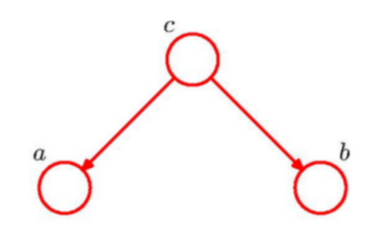
\includegraphics[scale=0.5]{2.png}}
			\end{figure}
			计算三个变量的联合概率:
			\[\text{因子分解:\quad}P(a,b,c) = P(c)P(a|c)P(b|c)\]
			\[\text{链式法则:\quad}P(a,b,c) = P(c)P(a|c)P(b|a,c)\]
			
			可得:\[P(b|c) = P(b|a,c)\Longrightarrow a\perp b|c\]
			
			该图的条件独立性:\textbf{若c被观测,则路径阻塞}(图论的说法,阻塞意味着独立)\\
			
			2.head to tail
			\begin{figure}[H]f
				\centering{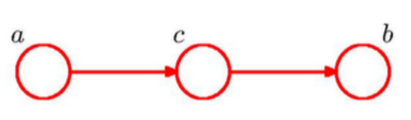
\includegraphics[scale=0.5]{3.png}}
			\end{figure}
			\textbf{若c被观测,则路径阻塞},$a\perp b|c$\\
				
			3.head to head
			\begin{figure}[H]
				\centering{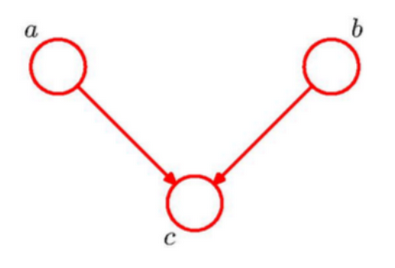
\includegraphics[scale=0.5]{4.png}}
			\end{figure}
			\textbf{若c被观测,则路径是通的,即a,b之间不独立}
			
			一个例子:
			\begin{figure}[H]
				\centering{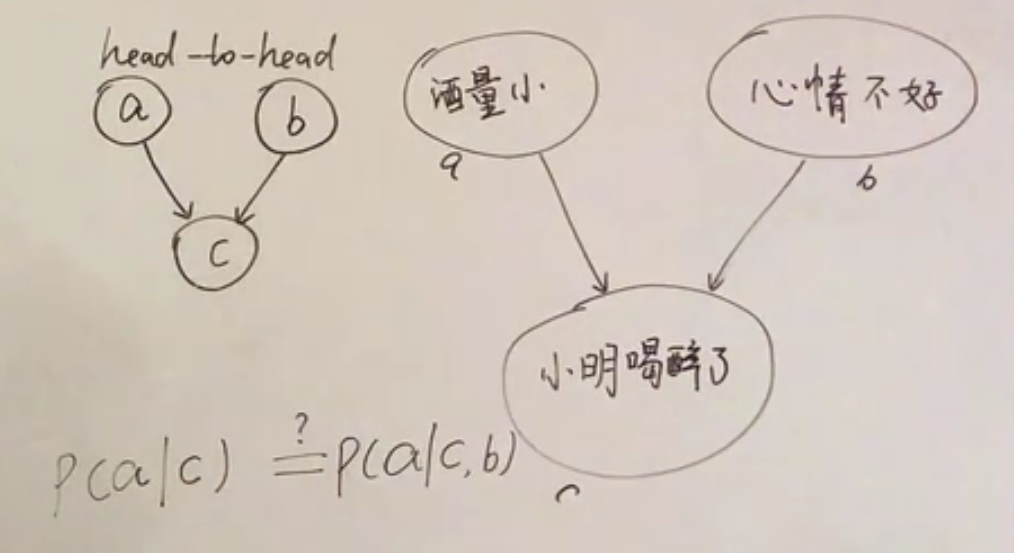
\includegraphics[scale=0.35]{5.png}}
			\end{figure}
			得知小明喝醉,推小明酒量小的概率$P(a|c)$应该是比较大的。
			
			得知小明喝醉且心情不好,推小明酒量小的概率$P(a|c,b)$就比上一种情况小了。因此a,b是相关的。
			
		\subsection{D划分(d-Separation)}
			1.集合A,B,C,通过tail to tail和head to tail结构连接,A到B的路径上的节点都\uline{必须}在C的内部。
			
			2.集合A,B,C,通过head to head结构连接,A到B的路径上的节点以及其后继节点都\uline{不能}在C的内部。
			
			满足上述两个要求,则$A\perp B|C$。即满足全局马尔可夫性。
			
			以下图为例,计算边缘概率$P(x_i|x_1,x_2,\cdots,x_{i-1},x_{i+1},\cdots, x_p)$:
			\begin{figure}[H]
				\centering{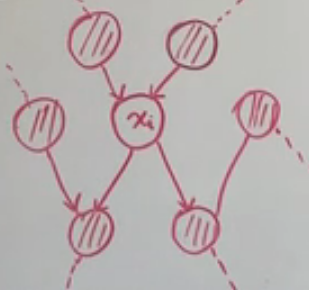
\includegraphics[scale=0.4]{6.png}}
			\end{figure}
			\[\begin{aligned}
			P(x_i|x_1,x_2,\cdots,x_{i-1},x_{i+1},\cdots, x_p) &= \frac{P(X)}{P(x_1,x_2,\cdots,x_{i-1},x_{i+1},\cdots, x_p)}\\
			&=\frac{P(X)}{\int P(X)dx_i}\\
			&=\frac{\prod_{j=1}^pP(x_j|x_{parent(j)})}{\int \prod_{j=1}^pP(x_j|x_{parent(j)})dx_i}\\
			&x_{parent(j)}\text{表示}x_i\text{的父节点们}
			\end{aligned}\]			
			
			可见$x_i$的边缘概率只与和它相关的一些节点有关,即上图中的打阴影的节点,$x_i$周围的一圈又叫马尔可夫毯。
			
			
	\section{Markov网络}	
		全局马尔可夫性:从节点集A中的节点到B中的节点的路径,都经过节点集C中的节点,则$A\perp B|C$。
		
		局部马尔可夫性:$a\perp \{\text{全集}-a-\text{邻居}\}|\text{邻居}$。
		
		成对马尔可夫性:$x_i\perp x_j|\{\text{全集}-x_i-x_j\}$ 
		
		团:图中节点的一个子集,其中任意两个节点有互相连接。
		
		极大团:在极大团中再加入一个节点就不够成团。
		
		因子分解(极大团的势函数相乘):
		\[P(X) = \frac{1}{Z}\prod_{i=1}^k \psi(x_{C_i})\]
		
		
		

			

		
			
			
\end{document}